\documentclass[usepdftitle=false,green]{beamer}
\beamertemplatenavigationsymbolsempty
\usepackage{beamerthemesplit}
\usepackage{graphics}
\usepackage{float}

%\usepackage[frenchb]{babel}
\usepackage[T1]{fontenc}
\usepackage[utf8]{inputenc}
\usepackage{lmodern}

\usepackage{amssymb,amsmath}

\usepackage{enumerate, graphicx}
\usepackage{eurosym}
\usepackage{comment}
\usetheme{Warsaw}
%\usefonttheme{serif} 
\usecolortheme{lily}
\usepackage{ gensymb }
\useinnertheme[shadow=true]{rounded}
\useoutertheme{infolines}

\usepackage{enumitem}
\usepackage{color}
\usepackage{multicol}
  
    
\title[Projet HPC]{\textbf{Décision de finales d'échecs}}

\author[M. Caristan \& A. Fernandez]{Mathis \textsc{Caristan} \& Alexandre \textsc{Fernandez}}

\institute[]{\textsc{UPMC}}
\date{28 Mars 2017}
%\begin{comment}
\newcommand{\nologo}{\setbeamertemplate{logo}{}} % command to set the logo to nothing
\logo{%
  \vspace*{-5ex}\makebox[0.98\paperwidth]{%
    %%\includegraphics[width=1cm,keepaspectratio]{pics/lpnhe.jpeg}%
    \hfill%
    %%\includegraphics[width=1cm,keepaspectratio]{pics/ATLAS.png}
  }%
}
%\end{comment}

%\usepackage[sorting=none, style=numeric, hyperref=auto]{biblatex}


%Centrer la table des matières
\usepackage{varwidth}    
\usepackage{etoolbox}
\makeatletter
\patchcmd{\beamer@sectionintoc}{%
  \hbox{\vbox{%
    \def\beamer@breakhere{\\}%
    \beamer@tocact{\ifnum\c@section=#1\beamer@toc@cs\else\beamer@toc@os\fi}{section in toc}}}%
}{%
  \hbox{%
    \def\beamer@breakhere{}%
    \beamer@tocact{\ifnum\c@section=#1\beamer@toc@cs\else\beamer@toc@os\fi}{section in toc}}%
}{}{}
\makeatother 

%Numerotation sans appendix
 \usepackage{etoolbox}
\makeatletter
\preto{\appendix}{%
  \patchcmd{\beamer@continueautobreak}{\refstepcounter{framenumber}}{}{}{}}
\makeatother


\begin{document}

{\nologo
\begin{frame}
\titlepage
\end{frame}
}

 \begin{frame}
 \frametitle{Table des matières}
\begin{center}
\begin{varwidth}{\textwidth}
\tableofcontents[sectionstyle=show,subsectionstyle=hide] 
\end{varwidth}
\end{center}
 \end{frame}
 
\section{Implémentation}
	\subsection{OpenMP}
\begin{frame}
    %\frametitle{Le LHC}
        \begin{center}
        \begin{itemize}
            \item[$\bullet$] \textbf{Idée : } Paralléliser la boucle \texttt{for} dans \texttt{evaluate}
            \item[$\bullet$] Profondeur max : 2 $\longrightarrow$ \textasciitilde 30 noeuds
            \item[$\bullet$] Deux choix d'implémentations possibles
                \begin{itemize}
                    \item[a$\degree$)] \texttt{parallel for} (plus simple)
                    \item[b$\degree$)] \texttt{task} (plus efficace)
            \end{itemize}
        \end{itemize}
            \begin{figure}
                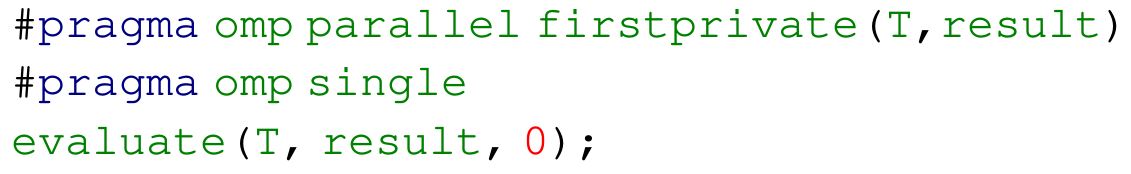
\includegraphics[scale=0.2]{pics/code1.png}
            \end{figure}
        \end{center}
\end{frame}

\begin{frame}
    \begin{center}
        \begin{figure}
            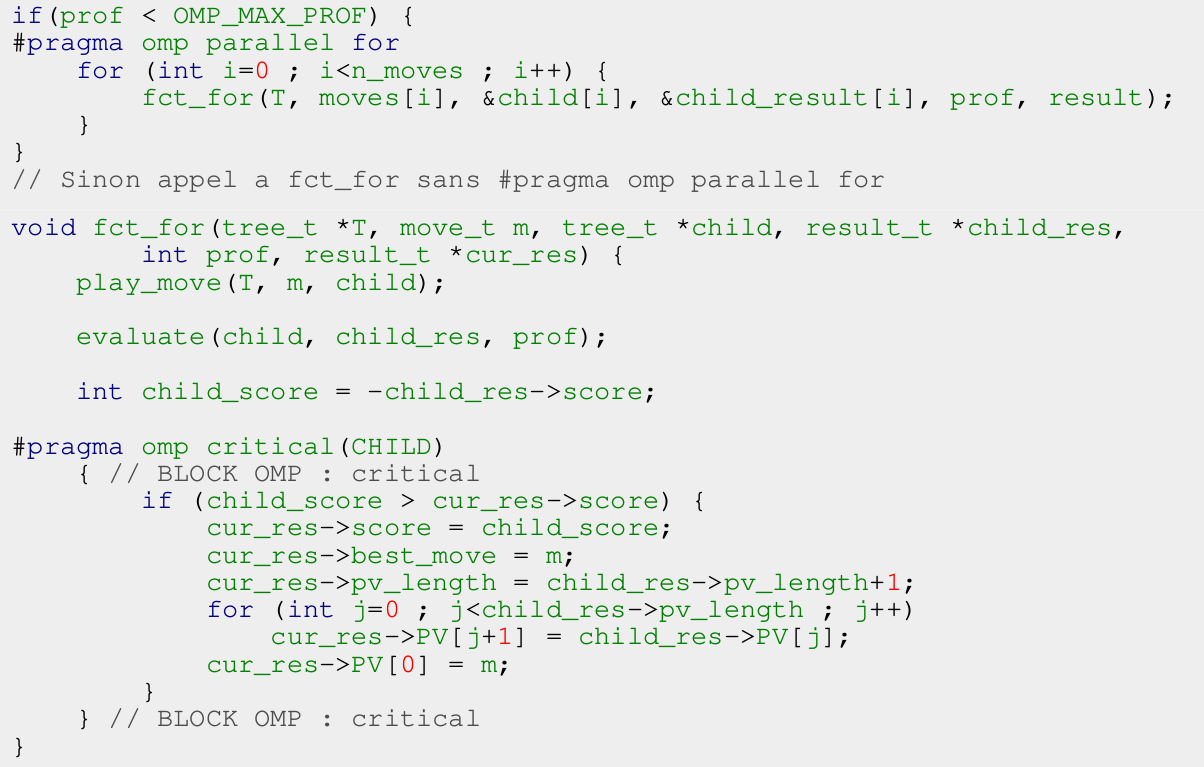
\includegraphics[scale=0.2]{pics/code2.png}
        \end{figure}
        \begin{itemize}
            \item[$\bullet$] Bloc \texttt{critical} pour protéger les accès concurents à cur\_res
            \item[$\bullet$] Factorisation du code dans la fonction \texttt{fct\_for}
        \end{itemize}
    \end{center}
\end{frame}


\begin{frame}
    \begin{itemize}
        \item[$\bullet$] \texttt{play\_move} et \texttt{evaluate} sont lancés dans des tâches
        \item[$\bullet$] Barrière de synchornisation à la fin du \texttt{for}
        \item[$\bullet$] Découpage de la boucle en deux zones, dont une seule est critique
    \end{itemize}
    \begin{center}
        \begin{figure}
            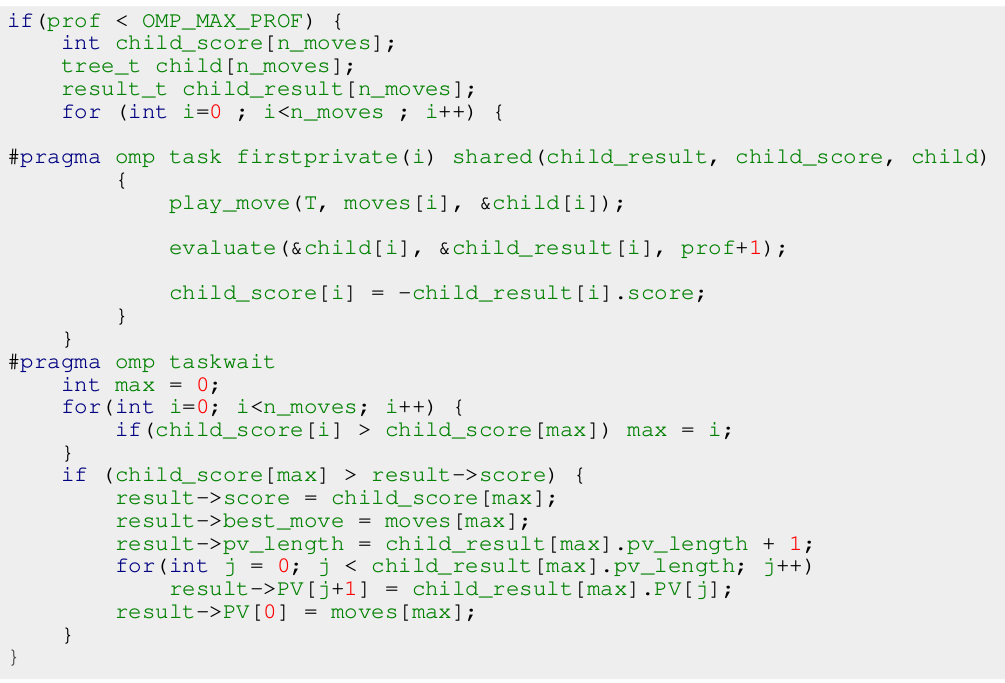
\includegraphics[scale=0.2]{pics/code3.png}
        \end{figure}
    \end{center}
\end{frame}

    \subsection{MPI}

\begin{frame}
    \begin{itemize}
        \item[$\bullet$] \textbf{Idée : } Atteindre une profondeur suffisante pour avoir une multiplicité de tâches intéressante.
        \item[$\bullet$] Pré-calcul (séquentiel) consistant à un parcours en largeur de l'arbre.
        \item[$\bullet$] \'Equilibrage de charge dynamique
        \item[$\bullet$] {\color{red} Réglages nécessaires selon les conditions d'utilisation}
    \end{itemize}
\end{frame}

\begin{frame}
	\frametitle{Simulation Monte-Carlo et données}
	\begin{figure}[t]
		\vspace{-5ex}
		%%\includegraphics[scale=0.33]{pics/hadronisation.png}
	\end{figure}
	\begin{itemize}
		\item[$\bullet$] Trois niveaux dans la simulation :
\textbf{Le niveau partonique, le niveau vrai ({\scriptsize ou niveau particules, niveau hadronique}) et le niveau reconstruit}.
		\item[$\bullet$] Les données ne donnent accès qu'au niveau
reconstruit.
		\item[$\bullet$] La simulation est utilisée dans la mesure de section efficace inclusive pour évaluer l'efficacité de la sélection.
	\end{itemize}
\end{frame}

\begin{frame}
	\frametitle{Sections efficaces}
	%\vspace{-7ex}
	\begin{columns}
		\begin{column}{8.2cm}
			{\small
			\begin{equation*}
				\sigma_{incl}(pp\rightarrow t\bar t) = \frac{N_{signal}^{hadronique}}{\epsilon_{t\bar t}^{incl} \cdot \mathcal L \cdot BR^{hadronique}}
			\end{equation*}
			}
			{\scriptsize
			\begin{tabular}{|l|l|}
				\hline
				Coupure & Variable \\
				\hline% \hline
				Préselection & $|\eta| < 2.4\:\&\:p_T > 25 GeV$\\
				%\hline
				Nombre de jets & $n_{jet} \geqslant 6$ \\
				%\hline
				Isolation des jets & $\Delta R(jet_i,jet_j) > 0.6$\\
				%\hline
				Impulsion transverse du $5^{ème}$ jet & $p_T^{jet5} > 65 GeV$\\
				%\hline
				{\color{blue}\'Etiquetage des jets }& {\color{blue}$n_{bjet} = 2$ }\\
				%\hline 
				Isolation des jets étiquetés & $\Delta R(b_1,b_2) > 1$\\
				%\hline
				Impulsion transverse du $6^{ème}$ jet & $p_T^{jet6} > 45 GeV$\\
				%\hline
				{\color{blue}Distance boson W - jet de B }&{\color{blue}$\star$ }\\
				\hline
			\end{tabular}
			}
		\end{column}
		\begin{column}{4.3cm}
			{\footnotesize \color{blue}
			L'étiquetage au niveau vrai correspond à une association avec un quark b au niveau partonique par proximité spatiale. Au niveau reconstruit, c'est un algorithme qui utilise les informations des détecteurs à pixels et du trajectographe.}
		\end{column}
	\end{columns}
	\begin{itemize}
		\item[$\bullet$] $\epsilon_{t\bar t}^{incl}$ déterminée grâce à la simulation. La section efficace inclusive dépend du modèle.
		\item[$\bullet$] \textbf{On cherche à \textit{minimiser} cette dépendance dans la section efficace fiducielle.}
		\item[$\bullet$] Les coupures doivent être adaptées et optimisées pour être appliquées au niveau vrai.
	\end{itemize}
\end{frame}



\section{Analyse}
{\nologo  
\begin{frame}
	\frametitle{Détermination des bonnes combinaisons de jets par une méthode de $\chi^2$}
	\vspace{-5ex}
	\begin{columns}
	\vspace{15ex}
		\begin{column}{8.5cm}
			La cinématique du processus permet de déterminer la bonne combinaison de jet pour chaque événement.
			{\scriptsize
			\begin{equation*}
				\chi^2 = \frac{ (m_{b_1j_1j_2}-m_t)^2 }{ \sigma_t^2 } + \frac{
		(m_{b_2j_3j_4}-m_t)^2 }{ \sigma_t^2 } + \frac{ (m_{j_1j_2}-m_W)^2 }{
		\sigma_W^2 } + \frac{ (m_{j_3j_4}-m_W)^2 }{ \sigma_W^2 }
			\end{equation*}
			\vspace{-7ex}
			$m_t = $ paramètre libre.
			}
		\end{column}
		\begin{column}{3cm}
			\vspace{1ex}
			\begin{figure}
				%%\includegraphics[scale=0.2]{pics/diagram.png}
			\end{figure}
		\end{column}
	\end{columns}
	\vspace{3ex}
	\begin{columns}
		\begin{column}{6.2cm}
			%%\includegraphics[scale=0.125]{pics/mw.png}
		\end{column}
		\begin{column}{6.2cm}
			%%\includegraphics[scale=0.125]{pics/mt.png}
		\end{column}
	\end{columns}
	$m_W, \sigma_W, \sigma_t$, sont déterminés à partir de distributions de masse au niveau hadronique de la simulation.
\end{frame}
}

\begin{frame}
	\frametitle{Fiabilité et amélioration du $\chi^2$}
	La méthode de $\chi^2$ peut être améliorée en utilisant l'information sur l'étiquetage des jets B.
	\begin{columns}
		\begin{column}{6.2cm}
			\'Ecart entre le minimum, et le second minimum du $\chi^2$.
			\begin{figure}
				\vspace{-4ex}
				%%\includegraphics[scale=0.13]{pics/deltaMinChi2.png}
			\end{figure}
		\end{column}
		\begin{column}{6.2cm}
			\'Ecart entre le minimum de $\chi^2$, et le $\chi^2$ de la bonne combinaison.
			\begin{figure}
				\vspace{-4ex}
				%%\includegraphics[scale=0.13]{pics/deltaBestChi2.png}
			\end{figure}
		\end{column}
	\end{columns}
	L'utilisation de l'étiquetage des jets donne de meilleurs résultats.\\
	\begin{itemize}
		\item[$\star$] Les jets de B sont choisis parmi les jets étiquetés. {\scriptsize (Au niveau vrai)}
		\item[$\star$] Les autres jets sont choisis parmi les jets non étiquetés.
	\end{itemize}	 
\end{frame}

\begin{frame}
	\frametitle{La coupure sur $\Delta R(b,W)$}
	La coupure ne garde que les événements qui vérifient
	\vspace{-1ex}	
	\begin{center}
		$ |\Delta R(b,W) - \langle \Delta R(b,W) \rangle | < 2\sigma_{\Delta R(b,W)}$\\
		$\Delta R(b,W) = \sqrt{(\eta_b-\eta_W)^2 + (\phi_b-\phi_W)^2}$
	\end{center}
	\vspace{-7ex}
	\begin{columns}
		\begin{column}{6.2cm}
			\begin{figure}
				%%\includegraphics[scale=0.13]{pics/DRBW.png}
			\end{figure}
			$\Delta R(b,W)$ déterminé en associant les jets au niveau vrai {\scriptsize(hadronique)} aux partons. %C'est à partir de cette distribution que sont déterminés les paramètres de la coupure.
		\end{column}
		\begin{column}{6.2cm}
			\begin{figure}
			    	%%\includegraphics[scale=0.13]{pics/DRBWchi2.png}
			\end{figure}
			$\Delta R(b,W)$ déterminé en utilisant la combinaison de jets obtenue grâce au $\chi^2$. %C'est sur cette distribution qu'on effectue la coupure.
		\end{column}
	\end{columns}
\end{frame}

	\subsection{Chevauchement}
\begin{frame}
	\frametitle{Chevauchement des sélections aux niveaux vrai et reconstruit - Exemple}
	\begin{columns}
		\begin{column}{8cm}
			\vspace{-5ex}
			\begin{figure}
				%\includegraphics[scale=0.25]{pics/c0_2.png}
			\end{figure}
	\begin{figure}
		\vspace{-2ex}
		\hspace{3ex}
		%\includegraphics[scale=0.21]{pics/overlap.png}
	\end{figure}
		\end{column}
		\begin{column}{4.5cm}
			\hspace{-15ex}	
			\begin{itemize}
				{\small
				\item 1 : \'Evenements présents uniquement dans la sélection au niveau vrai.
				\item 2 : \'Evenements présents dans les deux sélection (chevauchement).
				\item 3 : \'Evenements présents uniquement dans la sélection au niveau reconstruit.
				}
			\end{itemize}
		\end{column}
	\end{columns}
\end{frame}

\begin{frame}
	\frametitle{Chevauchement des sélections aux niveaux vrai et reconstruit aux différentes étapes de la sélection}
	\begin{figure}
		%\includegraphics[scale=0.18]{pics/c0.png}
	\end{figure}
	\begin{itemize}
		\item[$\bullet$] Toutes les coupures ont été optimisées.
		\item 
		\item
	\end{itemize}
\end{frame}
\begin{frame}[noframenumbering]
	\frametitle{Chevauchement des sélections aux niveaux vrai et reconstruit en fonction des coupures}
	\begin{figure}
		%\includegraphics[scale=0.18]{pics/c0-2.png}
	\end{figure}
	\begin{itemize}
		\item[$\bullet$] Toutes les coupures ont été optimisées.
		\item[$\bullet$] {\color{red} L'étiquetage et la dernière coupure ont un effet important sur le chevauchement}
	\end{itemize}
\end{frame}

\begin{frame}
	\frametitle{Optimisation}
	\begin{columns}
		\begin{column}{6.2cm}
			{\scriptsize
			\begin{tabular}{c|c|c}
				Coupure & \'Etape précédente & Effet \\
				\hline \hline
				\'Etiquetage & 47.37 & 24.68 \\
				Distance b-W & 23.47 & 12.39  \\
			\end{tabular}
			}
		\end{column}
		\begin{column}{6.2cm}
			\begin{itemize}
				{\footnotesize
				\item[$\bullet$] L'effet de l'étiquetage est grandement dû à un effet de détecteur.
				\item[$\bullet$] Plusieurs optimisations ont été testées pour la dernière coupure.
				}
			\end{itemize}	
		\end{column}
	\end{columns}
	\begin{columns}
		\begin{column}{9cm}
			\begin{figure}
				%\includegraphics[scale=0.28]{pics/opti.png}
			\end{figure}
		\end{column}
		\begin{column}{3.5cm}
			Les paramètres de la coupure {\scriptsize($\langle \Delta R(b,W) \rangle$ et $\sigma$)} changent en fonction de l'impulsion transverse du top.
		\end{column}
	\end{columns}
\end{frame}

\begin{frame}
	\frametitle{Factorisation}
	\begin{columns}
		\begin{column}{6.2cm}
			\begin{figure}
				%\includegraphics[scale=0.17]{pics/cutflow.png}
			\end{figure}
		\end{column}
		\begin{column}{6.2cm}
			\begin{itemize}
				\item[$\bullet$] Seule la coupure d'étiquetage est dominée effets de détecteurs.
			\end{itemize}
			Une possibilité pour la correction à la section efficace inclusive est de ne corriger que par l'efficacité des trois dernières coupures.
		\end{column}
	\end{columns}
	\begin{equation*}
		\epsilon_{t\bar t}^{truth} = \epsilon_{fidu} * \epsilon_{model} \qquad ; \qquad \epsilon_{fidu} = \epsilon_{blabel}*\epsilon_{isoB}*\epsilon_{\Delta R(b,W)}
	\end{equation*}
	\begin{equation*}
		\sigma_{fidu}(pp\rightarrow t\bar t) = \frac{N_{signal}^{had}}{\epsilon_{fidu} \cdot \mathcal L \cdot BR^{had}} = 2.13~\textup{pb}
	\end{equation*}
\end{frame}

\section*{Conclusion}
\begin{frame}
	\frametitle{Conclusion}
	 Ce stage a été le deuxième que j'ai fait en laboratoire de recherche : 
	\begin{itemize}
		\item[$\bullet$] Il a renforcé mon envie de faire de la recherche ainsi que ma passion pour la physique des particules.
		\item[$\bullet$] \c Ca a été l'occasion de me préparer à la thèse. J'ai également pu discuter avec les doctorants de mon bureau, ce qui a été particulièrement enrichissant.
		\item[$\bullet$] Le stage m'a permis de mettre en application mes connaissances de l'année, et renforcer des compétences techniques. \c Ca a également été l'opportunité d'acquérir un savoir-faire plus technique.
	\end{itemize}
\end{frame}
	




\end{document}
